\chapter{Results}
\label{chap:results}

In this chapter we will present our results from analyzing the data in the blockchain using the methods described in \cref{chap:metodology}.
Bitcoin has a testnet used for development and testing of experimental functionality, which the LN have been tested on for longer than it has been used on the mainnet. We have used both the testnet and the mainnet in the project; our reasoning for this is the LN on the testnet is larger, and people are testing a wide array of use cases, and functionality using testnet coins without any value; on the mainnet users have Bitcoin with value, perhaps resulting in more realistic user behaviour which could impacts the data generated.
By using both Bitcoin networks we will have one with more edge cases and more data, and one containing data more accurately reflecting normal user behaviour.
The testnet has its own blockchain which is publicly available in the same manner as the mainnet blockchian. Collecting data from the LN as discussed in \cref{sec:ln_analysis} was done in two intervals of one week each. Creating a snapshot of the network on each block for a week results in about 1000 blocks worth of data. This should be sufficient to verify our methods of identifying relevant LN transactions, and doing this twice allowed us to make adjustments after the results of the first interval.

\section{Method verification with LN data}

Comparing data from the LN with our data from the blockchain, provided us with results about the extent our identification methods was able to locate LN channels on the blockchain and to which degree. There was three sets of data was used in these comparisons: 
\begin{itemize}
    \item The set \( \alpha \) , containing channels from the LN closed during the capture interval. 
    \item The set \( \beta \), containing channels from the blockchain identified using timelocked redeem scripts,
    \item The set  \( \gamma \), containing potential channels identified on the blockchain using 2of2 multisig scripts.
\end{itemize}

As we stated previously a LN channel uses the P2WSH 2of2 multisig type for the on chain founding - closing output - input pair. In \cref{detection_ms} we discussed how this could be used to give us a set of potential transactions being related to LN channels. Because the on-chain channel transactions must be of this type the \( \gamma \) set is guaranteed to include all channels closed in the block interval used for the search. It also means that the two other sets will be subset of \( \gamma \). So the relations between the sets should be as follows:

\begin{equation} \label{eq:1}
      \alpha \subseteq \gamma, \hspace{10pt} \beta \subseteq \gamma, \hspace{10pt} \beta \subseteq \alpha  
\end{equation}

The two first relations is explained above and is always true for the systems in its current case. The last relation however, will not hold with our data, but ideally it should be true. For this to be the case our method with timelocked redeem scripts for identifying channels should not have any false positives-i.e., identify channels which is unrelated to the LN. Additionally we should also be able to discover all closed channels from the LN during the interval, meaning we would get the complete set of channels-i.e., \( \gamma \) contain all LN channels closed in the interval. While the timelocked scripts are very unique and therefore good for identifying channels, and theoretically one could get all LN channels by connection to the LN, this would only be true in a ideal world scenario. So as we will see with our data \( \beta \not\subseteq \alpha \), but keeping the relation in mind will be useful when analyzing the data.

\subsection{First Interval}

\begin{figure}[h]
    \centering
    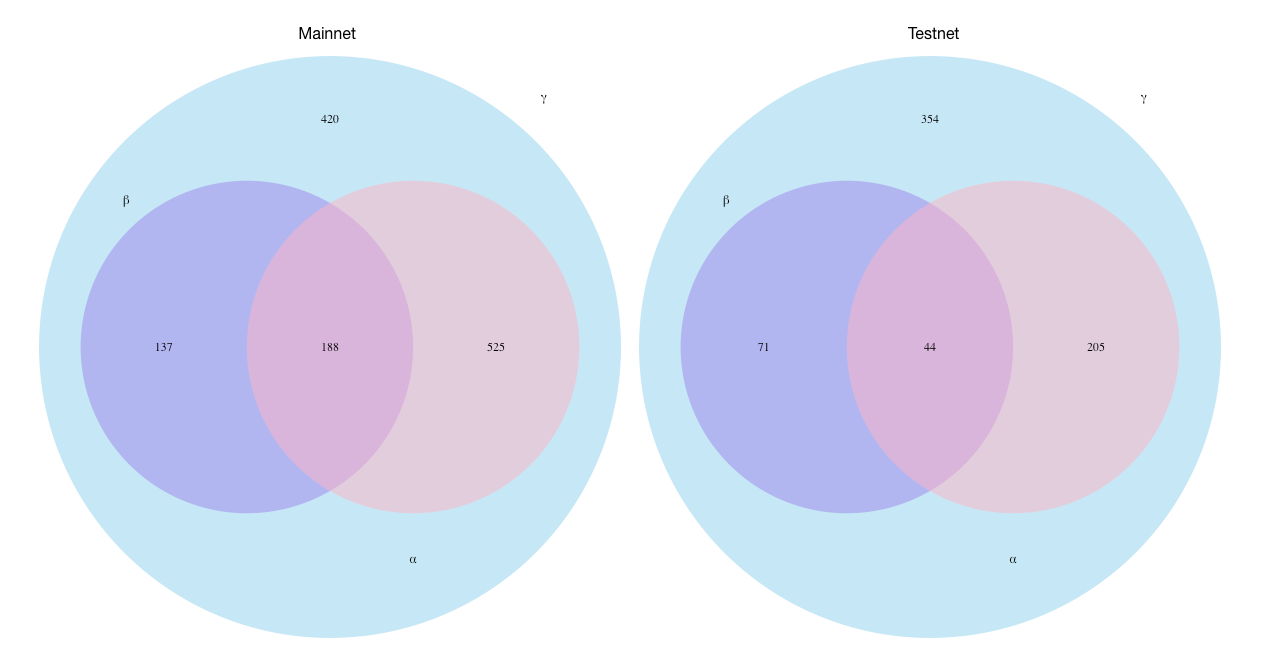
\includegraphics[width=16cm]{figures/graphs/venn_full1.png}
    \caption{Venn diagram of channel sets in interval one}
    \label{fig:venn_run1}
\end{figure}

The first collection interval on the mainnet had a length of 1151 blocks, found between block 517855 and 519005. Our modified LND implementation described in \cref{sec:ln_analysis} collected data from the LN and produced the set $\alpha$ containing 713 channels which where closed during this interval. The same interval on the blockchain was parsed two times, once identifying channels using timelocked redeem scripts, and a second time getting all potential channels using multisig identification. This resulted in a $\beta$ set containing 325 channels and a $\gamma$ set with 1270 channels shown on the left in \cref{fig:venn_run1} as a venn diagram. We can see how both $\beta$ and $\alpha$ is a subset of $\gamma$, but $\beta \not\subseteq \alpha$. The intersection $\beta \cap \alpha$ is the number of channels we identified using the timelocked method which was also found trough the LN node. On the mainnet this intersection was 188 which is 26.37\% of total channels in $\alpha$. This is reasonable as the method will only discover a channel if it has been unilaterally closed as we explained in \cref{sec:bc_analysis} and not if a channel is closed cooperatively which likely will happen more frequently. Taking the ideal world scenario $\beta \subseteq \alpha$ discussed above into account for this data, we have a large $\beta \backslash{} \alpha$ relative compliment of $\alpha$ in $\beta$ of 137, which is 42.15\% of the channels in $\beta$. Having a false positive this high is very unlikely because the uniqueness of the timelocked redeem scripts, so we made the assumption that these are actually LN channels which we have not been able to capture in our interaction with the LN. \todo{add for interval 2 more peers, and graph pruning theory}
Assuming the union $\alpha \cup \beta$ are all LN channels, the total number of LN channels closed in this interval would be 850. In turn this would entail that 66.93\% of 2of2 multisig transactions in our interval is lightning channels. For the testnet data this the percentage would be slightly lower with 47.48\%.
This is however not a upper limit as our $\alpha \cup \beta$ union is only channels unilaterally closed on the blockchain and channels that have been propagated to our node in the LN. If the notion that the relative compliment $\beta \backslash{} \alpha$ is unilaterally closed channels, which we have not been able to collect trough the LN, there should also be channels not closed unilaterally and therefore not discovered on the blockchain, which we similarly have not been able to collect trough the LN. 
Which would make the total channel count higher, and more of the 2of2 multisig transactions being channels, than is indicted in our data.

\subsection{Second Interval}

\begin{figure}[h]
    \centering
    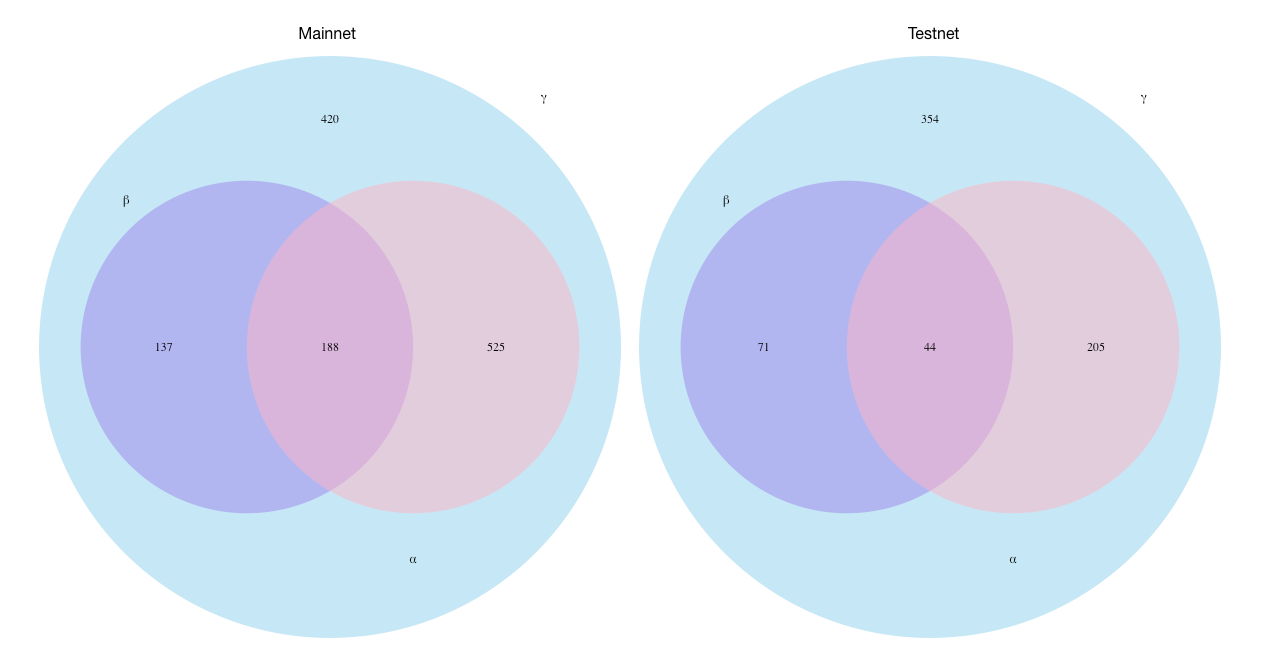
\includegraphics[width=16cm]{figures/graphs/venn_full1.png}
    \caption{Venn diagram of channel sets in interval one}
    \label{fig:venn_run2}
\end{figure}

\section{LN size}

We mentioned in \cref{subsec:information_ln} how using the fact that on-chain LN transactions used for channel creation has to be of the P2WSH type, to determine the maximum possible size of the LN. We have counted all unspent P2WSH outputs for each blockheight, in both the mainnet and the testnet. Our results is shown in \cref{fig:ln_size}, where we can see a distinct difference in the two networks: the mainnet has a more organic growth as a result of real world use, while the testnet graph is characterized by the testing which the network is used for. The sharp decline in unspent outputs on the mainnet at around block 505 000 can be explained by the sharp decline in fees for doing transactions at that time \cite{mempool_stats}, which incentivized users to consolidate their unspent outputs into fewer bigger ones. 

\begin{figure}[h]
    \centering
    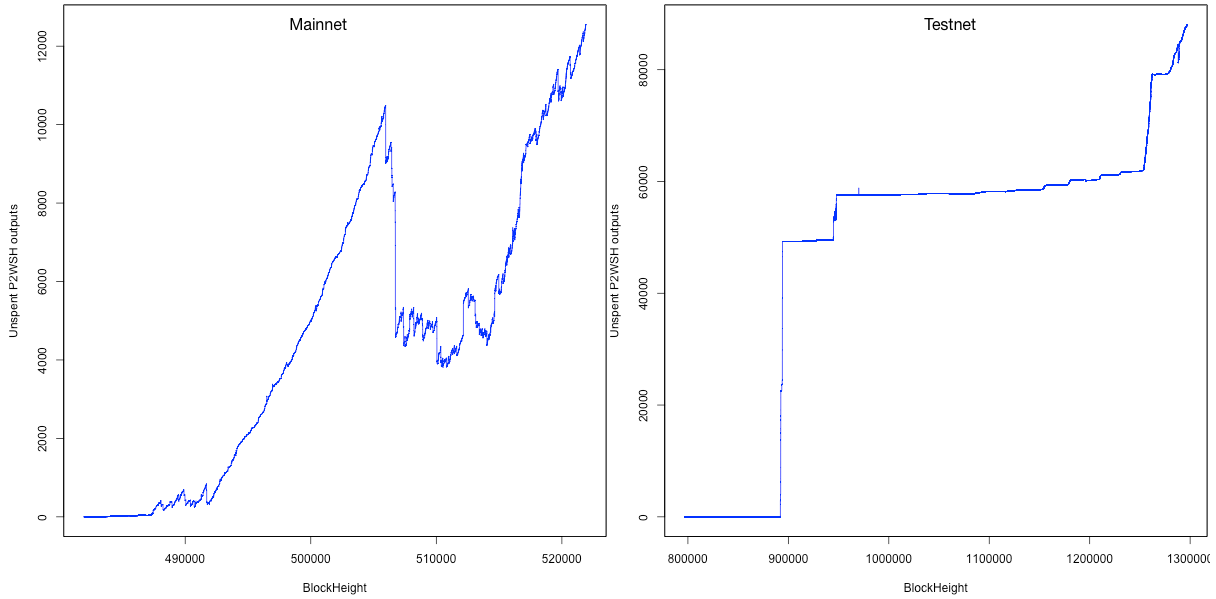
\includegraphics[width=16cm]{figures/graphs/ln_size_bc.png}
    \caption{Maximum size of the LN based on unspent P2WSH outputs on the blockchain}
    \label{fig:ln_size}
\end{figure}

While the unspent output count provides a concrete upper limit on the number of channels and therefore size of the LN, also wanted to know to which degree the amount of unspent P2WSH transactions was correlated to the size of the LN. It is clear that changes in the size of the LN will impact the number of P2WSH outputs/inputs, but there might be many other transactions not related to the LN having a larger impact. From the data we collected from the LN itself we constructed a channel count for each blockheight in the collection interval. Similarly we extracted the same block interval with the P2WSH output count from the blockchain. These two variables allowed us to compare the changes of number of channels in the LN and number of unspent P2WSH outputs. We used Kendall rank correlation coefficient \todo{check} on this data for the mainnet, which gave us a correlation coefficient of 0.73 indicating a strong positive correlation. The scatterplot for this can be seen in \cref{fig:correlation}.
We did the same for the testnet data which resulted in a coeficient of 0.45 which is only a moderate correlation. Both tests had the same p value: p < 2.2e-16.
\todo{include scatterplot for testnet?}

\begin{figure}[t]
    \centering
    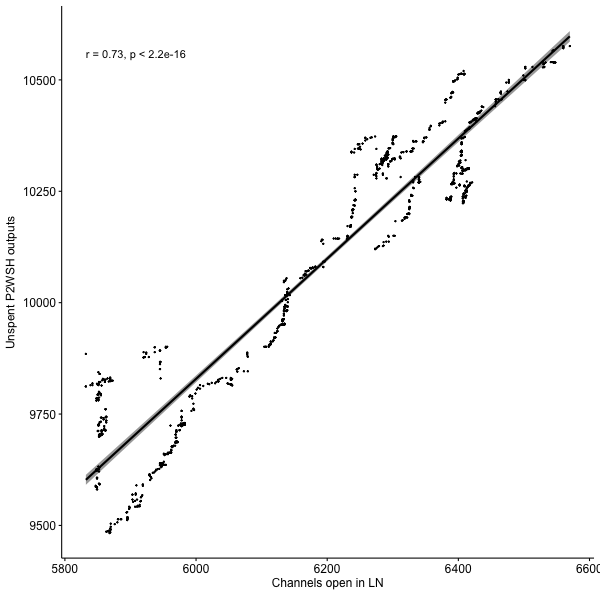
\includegraphics[width=10cm]{figures/graphs/channel_p2wsh_correlation_mainnnet.png}
    \caption{Correlation between unspent P2WSH outputs and channels open in the LN}
    \label{fig:correlation}
\end{figure}


\section{Channel Stats}

Using our software and the timelocked redeem scripts method for identifying channels we have parsed the blockchain on both mainnet and the testnet to the point before any P2WSH transactions and therefore channels. The result of this is data about every unilaterally closed channel that has existed. Statistics about the channels we identified can be found in \cref{subgraph_stats}. This include the number of channels fund and stats about their value and lifetime. The value of the channels is given in satoshis, with 100,000,000 satoshis being one Bitcoin. The One clear difference between the mainnet and testnet is the value used for each channel, as we briefly mentioned before coins on the testnet has no value to people, so it would be natural that they are more liberal when creating channels. 
\\

COMMENT: in table below i also have the same data from LN collection, so i can add in extra column so we can see if the stats are similar for bc data and ln.

\begin{table}[]
\centering
\caption{Value and lifetime for channels}
\label{subgraph_stats}
\begin{tabular}{|l|c|c|}
\hline
                                             & \textbf{Mainnet} & \textbf{Testnet} \\ \hline
\textbf{Total channels found}                & 3 400            & 7 755            \\ \hline
\textbf{Average Channel value}               & 412 647          & 7 000 458        \\ \hline
\textbf{Median channel value}                & 100 000          & 5 000 000        \\ \hline
\textbf{Standard Deviation Channel value}    & 1 296 102        & 7 096 572        \\ \hline
\textbf{Average channel lifetime}            & 1 438            & 2 282            \\ \hline
\textbf{Median channel lifetime}             & 602              & 396              \\ \hline
\textbf{Standard Deviation channel lifetime} & 2 017            & 5 545            \\ \hline
\end{tabular}
\end{table}

In \cref{channel_input_output} we see the distribution for the number of inputs and outputs to channels. These results are fairy similar for both networks, we should however note the percent of channels having two outputs in relation to the percent having only one input. For the mainnet the percent of channels having one input is 70\%, and the percent of channels only having one output is 71\%. As discussed in \cref{sec:bc_analysis} we cannot easily match input - output pairs to users in the channel, so these number either means that many channels does no off-chain transactions so the single input will be outputted back to owner, or all founds in the channel ends up at one of the entities. In the testnet column we can see how the single output percentage is lower compared to the single input percent, also the double output percent is higher than the double input. This indicates that many single founded channels ends up with splitting the value when they close, and as we stated in \cref{sec:bc_analysis} this enables us to say that off-chain transactions has taken place inside the channel.
This difference is also present when we checked how many channels had the same number of inputs as outputs. On the mainnet 60\% of channels found have the same number of inputs as outputs, while on the testnet this is 49\%. 
\\

COMMETN: planning on adding something about HTLC's. This would impact outputs of channels to give more meaning to these stats.
\begin{table}[]
\centering
\caption{Percentages of input - output count for channels}
\label{channel_input_output}
\begin{tabular}{|l|c|c|}
\hline
                                                                     & \textbf{Mainnet} & \textbf{Testnet} \\ \hline
\textbf{Channels with one input}             & 70.65            & 77.03            \\ \hline
\textbf{Channels with two inputs}            & 22.50            & 16.40            \\ \hline
\textbf{Channels with three inputs}          & 4.29             & 3.66             \\ \hline
\textbf{Channels with more than three inputs} & 2.56             & 2.91             \\ \hline
\textbf{Channels with one output}             & 71.74            & 52.79            \\ \hline
\textbf{Channels with two outputs}             & 27.47            & 44.52            \\ \hline
\textbf{Channels with three outputs}          & 0.65             & 1.92             \\ \hline
\textbf{Channels with more than three outputs} & 0.15             & 0.77             \\ \hline
\end{tabular}
\end{table}

\section{Clustering}

COMMENT: Below is the channel network graph from ln and the same graph created by linking channels found on the blockchain.
Results in blockchain graph is wrong, so will update when software method is fixed.

will also add table contaning number of channels linked, how many where linked using which heuristic, prevelance of key reuse, and talk about some outliers.

\begin{figure}[h]
    \centering
    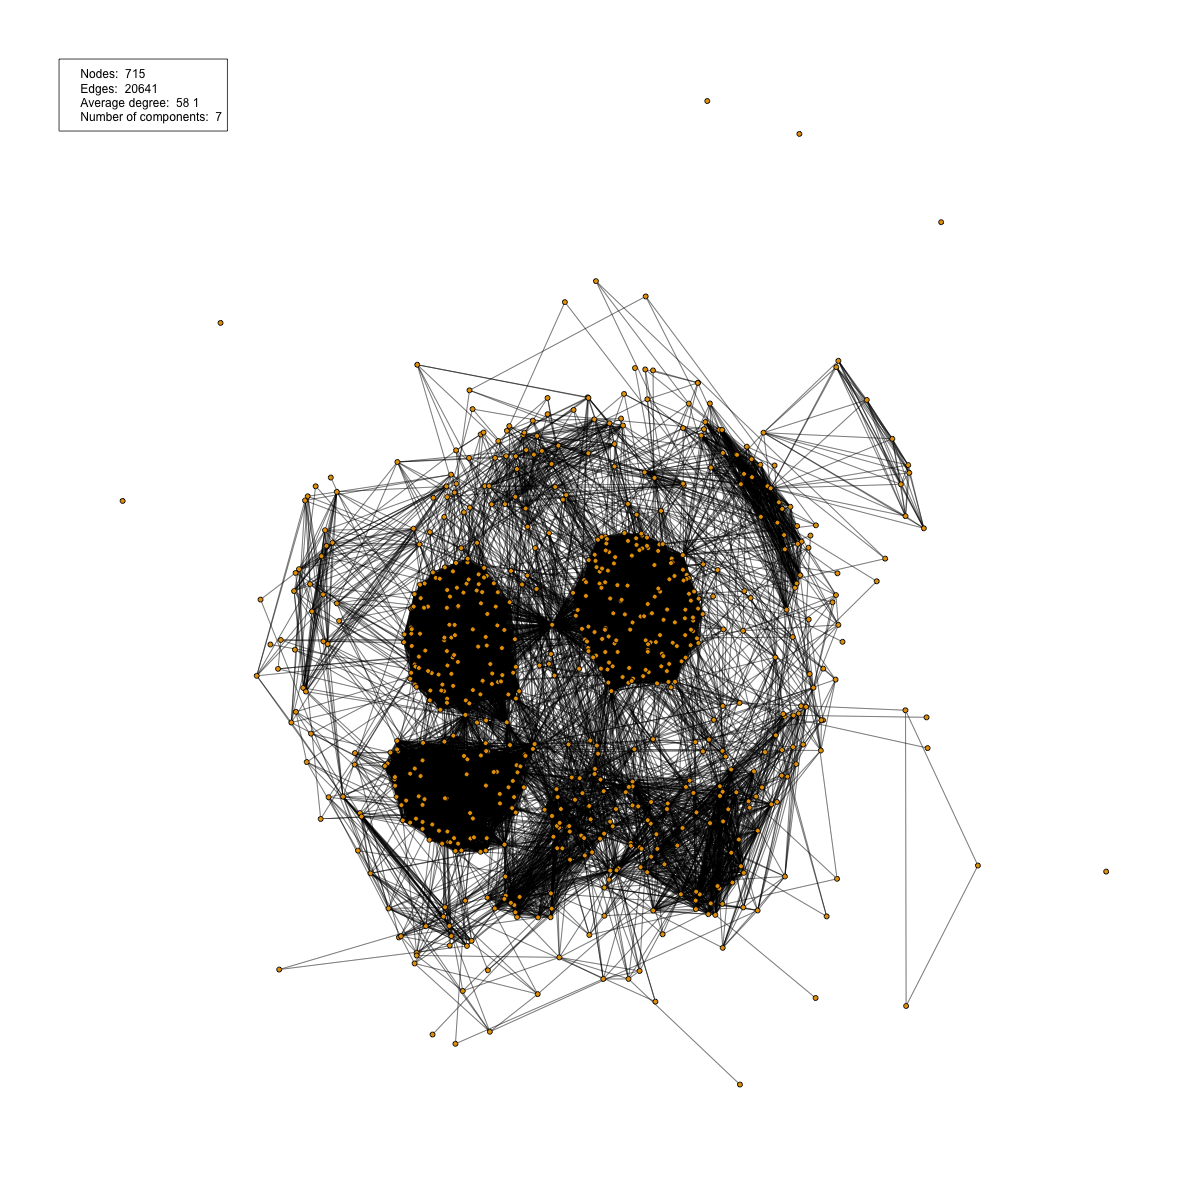
\includegraphics[width=14cm]{figures/graphs/cg_ln_mainnet_run1.png}
    \caption{Linked channels from LN mainnet run1}
    \label{fig:channelGraphLNTS}
\end{figure}

\begin{figure}[h]
    \centering
    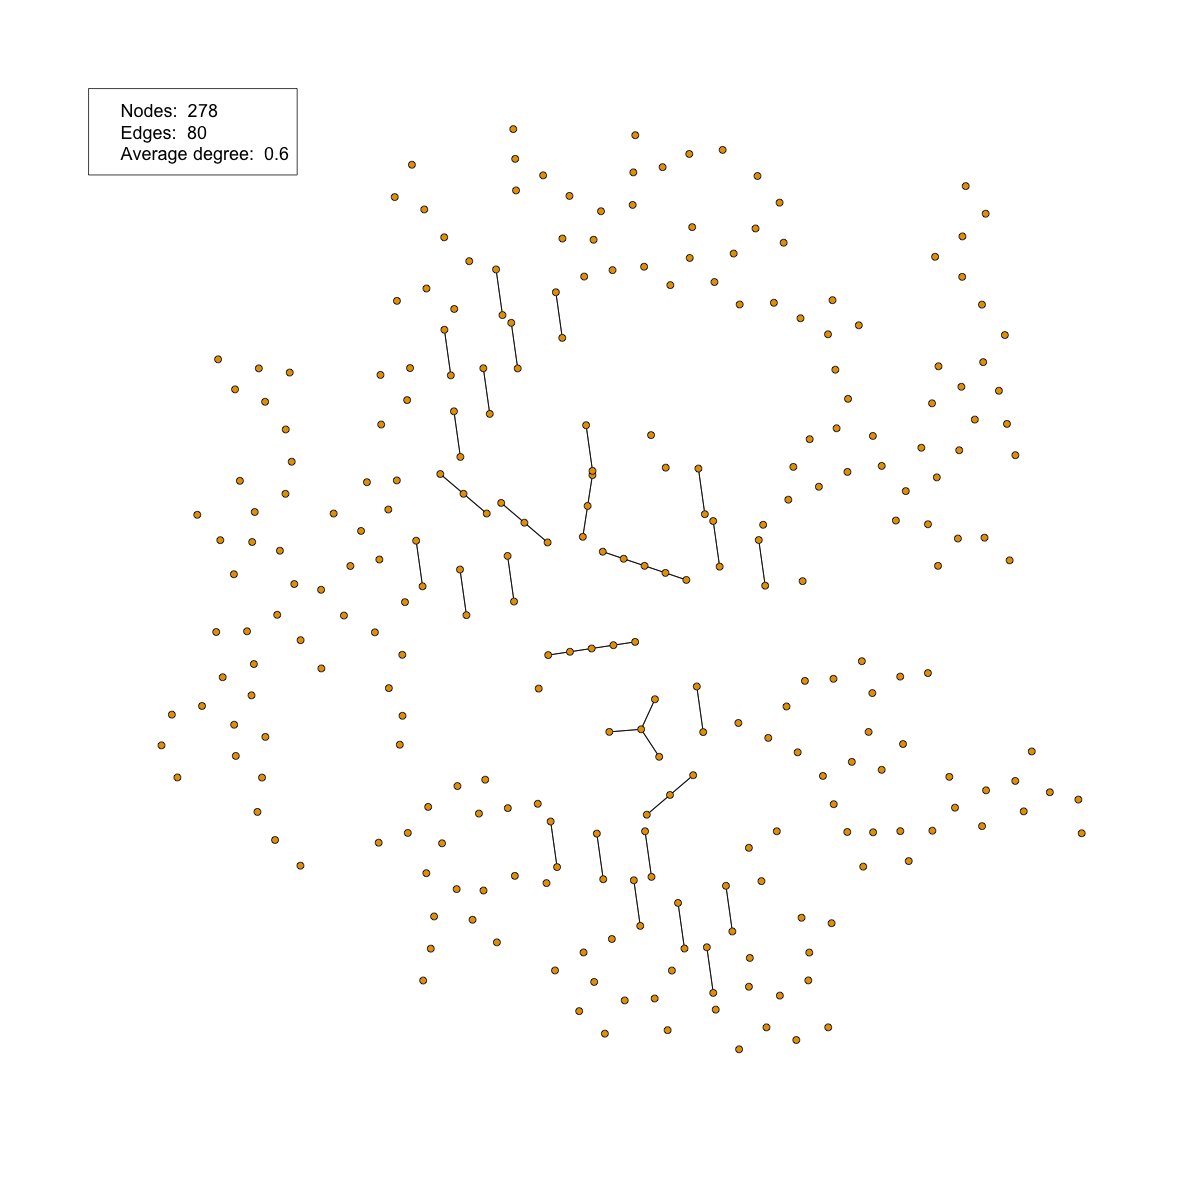
\includegraphics[width=14cm]{figures/graphs/cg_bc_mainnet_run1.png}
    \caption{Linked channels from BC mainnet run1}
    \label{fig:channelGraphLNTS}
\end{figure}